%%%%%%%%%%%%%%%%%%%%%%%%%%%%%%%%%%%%%%%%%%%%%%%%%%%%
% Document type, global settings, and packages
%%%%%%%%%%%%%%%%%%%%%%%%%%%%%%%%%%%%%%%%%%%%%%%%%%%%

\documentclass[12pt]{report}   %12 point font for Times New Roman
\usepackage{graphicx}  %for images and plots
\graphicspath{ {figures/} }
\usepackage[letterpaper, left=1.5in, right=1in, top=1in, bottom=1in]{geometry}
\usepackage[doublespacing]{setspace}  %use this package to set linespacing as desired
\usepackage{times}  %set Times New Roman as the font
\usepackage[explicit]{titlesec}  %title control and formatting
\usepackage[titles]{tocloft}  %table of contents control and formatting
\usepackage[backend=bibtex, sorting=none]{biblatex}  %reference manager
\usepackage[bookmarks=true, hidelinks]{hyperref}
\usepackage[page]{appendix}  %for appendices
\usepackage{rotating}  %for rotated, landscape images
\usepackage{amsmath}

% Custom definitions
\DeclareMathOperator*{\argmax}{arg\,max}

% For addiing subsubsubsection
\usepackage{titlesec}
\setcounter{secnumdepth}{4}
\titleformat{\paragraph}
{\normalfont\normalsize\bfseries}{\theparagraph}{1em}{}
\titlespacing*{\paragraph}
{0pt}{3.25ex plus 1ex minus .2ex}{1.5ex plus .2ex}


%%%%%%%%%%%%%%%%%%%%%%%%%%%%%%%%%%%
% Bibliography
%%%%%%%%%%%%%%%%%%%%%%%%%%%%%%%%%%%

%Add your bibliography file here
\bibliography{references}
% prevent certain fields in references from printing in bibliography
\AtEveryBibitem{\clearfield{issn}}
\AtEveryBibitem{\clearlist{issn}}

\AtEveryBibitem{\clearfield{language}}
\AtEveryBibitem{\clearlist{language}}

\AtEveryBibitem{\clearfield{doi}}
\AtEveryBibitem{\clearlist{doi}}

\AtEveryBibitem{\clearfield{url}}
\AtEveryBibitem{\clearlist{url}}

\AtEveryBibitem{%
  \ifentrytype{online}
    {}
    {\clearfield{urlyear}\clearfield{urlmonth}\clearfield{urlday}}}

%%%%%%%%%%%%%%%%%%%%%%
% Start of Document
%%%%%%%%%%%%%%%%%%%%%%

\begin{document}
%\doublespacing  %set line spacing

%%%%%%%%%%%%%%%%%%%%%%%%%%%%%%%%%%%%%
% Title Page
%%%%%%%%%%%%%%%%%%%%%%%%%%%%%%%%%%%%%
\currentpdfbookmark{Title Page}{titlePage}  %add PDF bookmark for this page
%% Define your thesis title, your name, your school, and your month and year of graduation here

\newcommand{\thesisTitle}{Joint Inference of Morphology and Syntax in Arabic}
\newcommand{\yourName}{Zeeshan Ali Sayyed}
\newcommand{\yourDepartment}{Computer Science}
\newcommand{\yourSchool}{Luddy School of Informatics, Computing and Engineering}
\newcommand{\university}{Indiana University}
\newcommand{\yourMonth}{May}
\newcommand{\yourYear}{2021}

%%%%%%%%%%%%%%%%%%%%%%%%%%%%%%%%%%%%%%%%%%%%%%%%%%%%%%%%%
% Do not edit these lines unless you wish to customize
% the template
%%%%%%%%%%%%%%%%%%%%%%%%%%%%%%%%%%%%%%%%%%%%%%%%%%%%%%%%%



\begin{titlepage}
\newgeometry{top=2in}
\begin{center}

{\large \MakeUppercase{\thesisTitle}}\\
\vspace{7\baselineskip}
\yourName\\
\vfill
Submitted to the faculty of the University Graduate School\\
in partial fulfillment of the requirements\\
for the degree\\
Doctor of Philosophy\\
in the Department of \yourDepartment,\\
\yourSchool,\\
\university\\
\yourMonth{} \yourYear{}

\end{center}
\restoregeometry
\end{titlepage}


%%%%%%%%%%%%%%%%%%%%%%%%%%%%%%%%%%%%%
% Approval Page
%%%%%%%%%%%%%%%%%%%%%%%%%%%%%%%%%%%%%
\pagenumbering{roman}
\setcounter{page}{2} % set the page number appropriately based on the number of intro pages
\newpage
%% Define your committee members. If you have less than 6, simple delete/comment the unused lines

\newcommand{\committeeChairpersonTypedName}{Dr. Sandra Kuebler}
\newcommand{\committeeChairpersonPostNominalInitials}{PhD}

\newcommand{\committeeMemberTwoTypedName}{Dr. David Crandall}
\newcommand{\committeeMemberTwoPostNominalInitials}{PhD}

\newcommand{\committeeMemberThreeTypedName}{Dr. Donald Williamson}
\newcommand{\committeeMemberThreePostNominalInitials}{PhD}

\newcommand{\committeeMemberFourTypedName}{Name}
\newcommand{\committeeMemberFourPostNominalInitials}{Post-Nominal Initials}

% Uncomment to add another committee member
%\newcommand{\committeeMemberFiveTypedName}{Name}
%\newcommand{\committeeMemberFivePostNominalInitials}{Post-Nominal Initials}

\newcommand{\myRule}{\rule{0.5\textwidth}{0.4pt}}

\newcommand{\approvalDay}{04}
\newcommand{\approvalMonth}{05}
\newcommand{\approvalYear}{2021}

%%%%%%%%%%%%%%%%%%%%%%%%%%%%%%%%%%%%%%%%%%%%%%%%%%%%%%%%%
% Do not edit these lines unless you wish to customize
% the template
%%%%%%%%%%%%%%%%%%%%%%%%%%%%%%%%%%%%%%%%%%%%%%%%%%%%%%%%%


\newgeometry{left=1in}

\begin{center}
 
Accepted by the Graduate Faculty, Indiana University, in partial fulfillment of the requirements for the degree of Doctor of Philosophy.

\end{center}

\vspace{2\baselineskip}

\ifdefined\committeeMemberFourTypedName
Doctoral Committee\\

\null\hfill \myRule\\
\null\hfill \committeeChairpersonTypedName, \committeeChairpersonPostNominalInitials\\
\null\hfill \myRule\\
\null\hfill \committeeMemberTwoTypedName, \committeeMemberTwoPostNominalInitials\\
\null\hfill \myRule\\
\null\hfill \committeeMemberThreeTypedName, \committeeMemberThreePostNominalInitials\\
\null\hfill \myRule\\
\null\hfill \committeeMemberFourTypedName, \committeeMemberFourPostNominalInitials\\

\ifdefined\committeeMemberFiveTypedName
\null\hfill \myRule\\
\null\hfill \committeeMemberFiveTypedName, \committeeMemberFivePostNominalInitials\\
\fi

\fi
\vfill
Date of Defense: \approvalMonth/\approvalDay/\approvalYear
\restoregeometry


%%%%%%%%%%%%%%%%%%%%%%%%%%%%%%%%%%%%%
% Copyright
%%%%%%%%%%%%%%%%%%%%%%%%%%%%%%%%%%%%%
\newpage
%%%%%%%%%%%%%%%%%%%%%%%%%%%%%%%%%%%%%%%%%%%%%%%%%%%%%%%%%
% Do not edit these lines unless you wish to customize
% the template
%%%%%%%%%%%%%%%%%%%%%%%%%%%%%%%%%%%%%%%%%%%%%%%%%%%%%%%%%

\clearpage
\begin{center}

\vspace*{\fill}
Copyright \copyright{} \yourYear{}\\
\yourName
\vspace*{\fill}

\end{center}
\clearpage


%%%%%%%%%%%%%%%%%%%%%%%%%%%%%%%%%%%%%
% Dedication
%%%%%%%%%%%%%%%%%%%%%%%%%%%%%%%%%%%%%
\newpage
% Define your dedication statement here

\newcommand{\yourDedication}{A great dedication goes here.}

%%%%%%%%%%%%%%%%%%%%%%%%%%%%%%%%%%%%%%%%%%%%%%%%%%%%%%%%%
% Do not edit these lines unless you wish to customize
% the template
%%%%%%%%%%%%%%%%%%%%%%%%%%%%%%%%%%%%%%%%%%%%%%%%%%%%%%%%%

\begin{center}

\vspace*{\fill}
\yourDedication\\
\vspace*{\fill}

\end{center}

%%%%%%%%%%%%%%%%%%%%%%%%%%%%%%%%%%%%%
% Acknowledgments
%%%%%%%%%%%%%%%%%%%%%%%%%%%%%%%%%%%%%
\newpage
\phantomsection
\addcontentsline{toc}{chapter}{Acknowledgements}
\begin{centering}
\textbf{ACKNOWLEDGEMENTS}\\
\vspace{\baselineskip}
\end{centering}

%Insert your dedication text here
\emph{Note}: Write this page at the very end



%%%%%%%%%%%%%%%%%%%%%%%%%%%%%%%%%%%%%
% Abstract
%%%%%%%%%%%%%%%%%%%%%%%%%%%%%%%%%%%%%
\newpage
\phantomsection
\addcontentsline{toc}{chapter}{Abstract}
%%%%%%%%%%%%%%%%%%%%%%%%%%%%%%%%%%%%%%%%%%%%%%%%%%%%%%%%%
% Do not edit these lines unless you wish to customize
% the template
%%%%%%%%%%%%%%%%%%%%%%%%%%%%%%%%%%%%%%%%%%%%%%%%%%%%%%%%%
\newgeometry{left=1in}

\begin{center}

\yourName\\
\MakeUppercase{\thesisTitle}

\end{center}

\vspace{1.5\baselineskip}

%Insert your abstract here
Lorem ipsum dolor sit amet, consectetur adipiscing elit, sed do eiusmod tempor incididunt ut labore et dolore magna aliqua. Ut enim ad minim veniam, quis nostrud exercitation ullamco laboris nisi ut aliquip ex ea commodo consequat. Duis aute irure dolor in reprehenderit in voluptate velit esse cillum dolore eu fugiat nulla pariatur. Excepteur sint occaecat cupidatat non proident, sunt in culpa qui officia deserunt mollit anim id est laborum.



\ifdefined\committeeMemberFourTypedName

\null\hfill \myRule\\
\null\hfill \committeeChairpersonTypedName, \committeeChairpersonPostNominalInitials\\
\null\hfill \myRule\\
\null\hfill \committeeMemberTwoTypedName, \committeeMemberTwoPostNominalInitials\\
\null\hfill \myRule\\
\null\hfill \committeeMemberThreeTypedName, \committeeMemberThreePostNominalInitials\\
\null\hfill \myRule\\
\null\hfill \committeeMemberFourTypedName, \committeeMemberFourPostNominalInitials\\

\ifdefined\committeeMemberFiveTypedName
\null\hfill \myRule\\
\null\hfill \committeeMemberFiveTypedName, \committeeMemberFivePostNominalInitials\\
\fi

\fi
\restoregeometry


%%%%%%%%%%%%%%%%%%%%%%%%%%%%%%%%%%%%%
% Table of Contents
%%%%%%%%%%%%%%%%%%%%%%%%%%%%%%%%%%%%%

% Format for Table of Contents
\renewcommand{\cftchapdotsep}{\cftdotsep}  %add dot separators
\renewcommand{\cftchapfont}{\bfseries}  %set title font weight
\renewcommand{\cftchappagefont}{}  %set page number font weight
\renewcommand{\cftchappresnum}{Chapter }
\renewcommand{\cftchapaftersnum}{:}
\renewcommand{\cftchapnumwidth}{5em}
\renewcommand{\cftchapafterpnum}{\vskip\baselineskip} %set correct spacing for entries in single space environment
\renewcommand{\cftsecafterpnum}{\vskip\baselineskip}  %set correct spacing for entries in single space environment
\renewcommand{\cftsubsecafterpnum}{\vskip\baselineskip} %set correct spacing for entries in single space environment
\renewcommand{\cftsubsubsecafterpnum}{\vskip\baselineskip} %set correct spacing for entries in single space environment

%format title font size and position (this also applys to list of figures and list of tables)
\titleformat{\chapter}[display]
{\normalfont\bfseries\filcenter}{\chaptertitlename\ \thechapter}{0pt}{\MakeUppercase{#1}}

\renewcommand\contentsname{Table of Contents}
\currentpdfbookmark{Table of Contents}{TOC}
\begin{singlespace}
\tableofcontents
\end{singlespace}


\clearpage

%%%%%%%%%%%%%%%%%%%%%%%%%%%%%%%%%%%%%
% List of figures and tables
%%%%%%%%%%%%%%%%%%%%%%%%%%%%%%%%%%%%%
\phantomsection
\addcontentsline{toc}{chapter}{List of Tables}
\begin{singlespace}
\setlength\cftbeforetabskip{\baselineskip}  %manually set spacing between entries
\listoftables
\end{singlespace}

\clearpage

\phantomsection
\addcontentsline{toc}{chapter}{List of Figures}
\begin{singlespace}
\setlength\cftbeforefigskip{\baselineskip}  %manually set spacing between entries
\listoffigures
\end{singlespace}

\clearpage

%%%%%%%%%%%%%%%%%%%%%%%%%%%%
%
% Chapters
%
%%%%%%%%%%%%%%%%%%%%%%%%%%%%

%%%%%%%%%%%%%%%%%%%%%%
% formatting
%%%%%%%%%%%%%%%%%%%%%%

% resume page numbering for rest of document
\clearpage
\pagenumbering{arabic}
\setcounter{page}{1} % set the page number appropriately

% Adjust chapter title formatting
\titleformat{\chapter}[display]
{\normalfont\bfseries\filcenter}{\MakeUppercase\chaptertitlename\ \thechapter}{0pt}{\MakeUppercase{#1}}  %spacing between titles
\titlespacing*{\chapter}
  {0pt}{0pt}{30pt}	%controls vertical margins on title
  
% Adjust section title formatting
\titleformat{\section}{\normalfont\bfseries}{\thesection}{1em}{#1}

% Adjust subsection title formatting
\titleformat{\subsection}{\normalfont\bfseries}{\thesubsection}{1em}{#1}

% Adjust subsubsection title formatting
\titleformat{\subsubsection}{\normalfont\itshape}{\thesubsubsection}{1em}{#1}

%%%%%%%%%%%%%%%%
% Chapter 1
%%%%%%%%%%%%%%%%

\chapter{Introduction and Background}

This is only a placeholder. This chapter should be written at the very end.

Parsing is an important problem in natural language processing. It involves deducing the linguistic structure of a given piece of text or sentence. In fact, parsing is a very broad term and can refer to its many different types, namely: syntactic, semantic or discourse. While semantic parsing deals with the representation of the meaning of the given piece of text, discourse parsing attempts to capture the relations between the different sentences of the text. Syntactic parsing, on the other hand, involves analyzing and assigning syntactic structure to a sentence in the form of syntactic representations called parse trees. The focus of thesis will chiefly be on syntactic parsing and its associated problems.

Syntactic parsing is a fundamental task of natural language processing, which forms a base on which many secondary tasks are built. Parse trees or syntactic representations produced by syntactic parsing can be used directly in tasks such as grammar checking. Moreover, they are used as intermediate structures in a variety of other tasks like machine translation, semantic analysis, information retrieval and question answering. For instance, to answer a wh-question like `\textit{Who did this?}' based on a given sentence, it is important to know what is the subject or the doer of the activity in that sentence. 

A corpus in which every sentence is syntactically annotated with a parse tree is called a treebank. A treebank typically consists of thousands of sentences drawn from a variety of sources, which are manually annotated with correct parse trees by humans. A wide variety of treebanks have been created for various languages like English, Arabic, Chinese, Czech, etc. The Penn Treebank Project, for instance, has treebanks from the Brown, Switchboard, Air Traffic Information System(ATIS) and the Wall Street Journal corpora of English \cite{jurafsky2014speech}. These treebanks play an important role in empirical investigations of various statistical phenomena and have considerably helped in the development of many parsers and parsing techniques over the past two decades. In fact, manually annotated treebanks allow syntactic parsing to be treated as a supervised machine learning problem. The sentences act as the independent variable $(X \in \mathcal{X})$ which are mapped to the parse trees, which act as the target or dependent variable $(y \in Y)$. Since the parse trees represent a complex structure and not just a simple class label or a number, parsing is actually viewed as structured prediction problem. The goal of this problem find the mapping function $f: \mathcal{X} \rightarrow \mathcal{Y}$.



%%%%%%%%%%%%%%%%
% Chapter 2
%%%%%%%%%%%%%%%%

\chapter{Literature Survey}

The outline of the chapter should be as follows:


English is the most heavily studied language by the NLP community and hence most of the tools for syntactic analysis have been developed keeping English and its treebanks in consideration. The techniques which have been developed for English do not naturally extend to many other languages like German, Hindi, Hebrew, Arabic, etc \cite{tsarfaty2010statistical}. These languages belong to a different class and are known as morphologically rich languages (MRLs). In this research question, I want to explore techniques that can be used for constituency parsing of MRLs. We will begin by understanding what are MRLs and what properties distinguish them from English in section \ref{sec:mrl}. In section \ref{sec:joint}, we will look at why joint morphological and syntactic analysis is important for MRLs and in section \ref{sec:lattice}, we will look at how it is done using lattices of part-of-speech tags.

\section{Morphologicall Rich Languages}
\subsection{What are MRLs?}
\label{sec:mrl}

A morpheme is the minimal meaning-bearing unit in a language. Multiple morphemes can be combined together to form new words in many different ways such as inflection, derivation, and cliticization. In NLP, morphology is the study of the way the words are built by the combination of one or more morphemes \cite{Jurafsky:2009:SLP:1214993}. A given word could thus contain multiple syntactic constituents with different syntactic functions. In relation to this, syntactic parsing operates at a higher level and uncovers the role of individual syntactic constituents and also the relations between various constituents. In a configurational language such as English, such syntactic information is conveyed through the order of constituents or words in the sentence. On the contrary, morphologically rich languages are those languages which convey such information by word formation (via inflection, cliticization, etc.) instead of word order \cite{seddah2013overview}. For instance, subject-predicate dependency is revealed by agreement on number and gender expressed by word morphology instead of their relative positions in the sentence. Owing to the above fundamental difference, MRLs tend to have a relatively \textit{free word order} i.e. the words in a sentence are free to change their positions without changing the meaning of the sentence. The non-rigid structure of parse trees owing to the free word order and morphological ambiguity due to a rich morphology are the major challenges of parsing MRLs. As has been pointed earlier, boundaries of constituents of the syntactic structure need not coincide with word boundaries as it happens in English.

\subsection{Joint inference of morphology and syntax}
\label{sec:joint}
In a typical NLP pipeline for English, first, the morphological analysis of the words of the sentence is performed which is followed by labelling the constituents with part-of-speech tags and eventually followed by syntactic parsing. But MRLs, owing to their nature, render such a pipeline ineffective. As was mentioned in the previous section, the boundaries of constituents need not coincide with word boundaries, as words can be made up multiple morphemes. Moreover, due to the existence of discontinuous constituents in MRLs, each of the constituents can play a variety of different syntactic roles. It has been pointed out by \cite{tsarfaty:2006} that there is a lot of ambiguity in each of the steps in the pipeline for MRLs. To disambiguate syntactic analysis (parsing), information needs to flow from the morphological analysis (segmentation) towards it, whereas, for disambiguation of morphological analysis, information needs to flow from syntactic analysis towards it. The common ground which connects these two tasks is part-of-speech tagging. Thus for an effective system, information should flow in both directions: $segmentation \rightarrow tagging \rightarrow parsing$ as well as $parsing \rightarrow tagging \rightarrow segmentation$.

This can be achieved by performing a joint morphological and syntactic analysis. Consider a sentence of $m$ words represented as  $w_1^m$. Let this sentence be segmented in $n$ constituents represented by $s_1^n$. Let the sequence of tags associated with every segment be denoted by $t_1^n$. Finally, let the parse tree be denoted by $\pi$. The goal of the joint morpho-syntactic analysis is shown in equation \ref{eq:joint_1}. This can be broken down into various components as shown in equation \ref{eq:joint_2}

\begin{align}
    \label{eq:joint_1}
    {\langle \pi, t_1^n, s_1^n \rangle}^* &= \argmax_{\langle \pi, t_1^n, s_1^n \rangle} p({\langle \pi, t_1^n, s_1^n \rangle} | w_1^m) \\
    &= \argmax_{\langle \pi, t_1^n, s_1^n \rangle} \underbrace{p(\pi \mid t_1^n, s_1^n, w_1^m)}_\text{parsing} \underbrace{p(t_1^n \mid s_1^n, w_1^m)}_\text{tagging} \underbrace{p(s_1^n \mid w_1^m)}_\text{segmentation}
    \label{eq:joint_2}
\end{align}

\cite{cohen:smith:2007} proposed a system that performs joint inference using factored models for morphology and syntax, which are designed and trained individually.


\subsection{Lattice parsing}
\label{sec:lattice}

Consider a word $w$ which has two possible segmentations i.e. it can either be segmented as $(s_1, s_2)$ with corresponding POS tags $(t_1, t_2)$ or the entire word can act as a single segment $s_3$ with $t_3$ as the corresponding POS tag. Information which tells us which what the right segmentation is, lies in the syntactic analysis of the sentence. But, at the same time, we need the right segmentation in order to perform the right syntactic analysis. In a traditional sequential analysis, either the segmentation having greater likelihood (as calculated from the treebank) will be preferred or the model will just take into account their likelihoods without the syntactic context. To avoid this, \cite{goldberg:tsarfaty:2008} introduced the idea of lattice parsing, in which, instead of parsing over a fixed input sentence, the parser operates on a structure of all possible segmentations called the lattice.

The idea of representing ambiguity as lattice structures is inspired by the speech recognition community \cite{chappelier:etal:1999} where it represents the different possible sentences resulting from an utterance based on the acoustic model. In our situation, it represents all possible segmentation and corresponding POS tags for a given sentence. A path through the lattice represents one possible morphological segmentation of the given sentence. Consider an example lattice representation of the Hebrew phrase \textit{bclm hneim} as presented by \cite{goldberg:tsarfaty:2008} as shown in figure \ref{fig:lattice}.

\begin{figure}[htb]
    \centering
    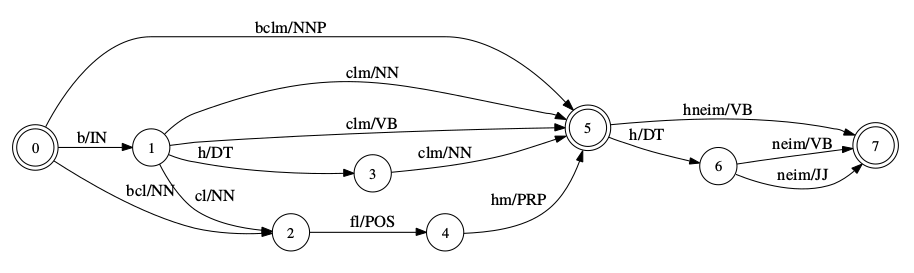
\includegraphics[scale=0.47]{lattice}
    \caption{The Lattice for the Hebrew phrase \textit{bclm hneim}}
    \label{fig:lattice}    
\end{figure}

The traditional PCYK algorithm for constituency parsing was extended to accept lattice inputs and to search over all lattice paths instead of just words in a sentence. \cite{goldberg:elhadad:2011} and \cite{green:manning:2010} have shown that doing so increases the parsing accuracy for Hebrew and Arabic respectively. In shift-reduce constituency parsing, most work either assume that they have access to gold segmentation and tagging labels or perform segmentation and tagging as a precursor to parsing, which hurts the parsing accuracies. The standard shift-reduce parsing algorithm for constituency parsing can also be modified to incorporate tag-lattices as inputs instead of plain sentences. It has been done for Chinese by \cite{wang2014joint} whereas \cite{mi2015shift} used for English and Chinese.

%%%%%%%%%%%%%%%%
% Chapter 3
%%%%%%%%%%%%%%%%

\chapter{Data and Methodology}

\section{Data}
\subsection{Penn Arabic Treebank}
\subsection{SPMRL Splits}
\subsection{Classical Arabic Data from Doha Project}

\section{Methodology}
\subsection{Deep Learning Methods for NLP}
\subsubsection{Word Embeddings}
\subsubsection{LSTMs}
\subsubsection{Transformers}

\subsection{Multitask Learning}
\subsubsection{Heirarchical Multitask Learning}


%%%%%%%%%%%%%%%%
% Chapter 4
%%%%%%%%%%%%%%%%

\chapter{Experiments}

\section{Joint Segmentation and Orthography Standardization}

\section{Part of Speech Tagging}

\section{Parsing}

%%%%%%%%%%%%%%%%
% Chapter 5
%%%%%%%%%%%%%%%%

\chapter{Discussion and Conclusion}
Lorem ipsum dolor sit amet, consectetur adipiscing elit, sed do eiusmod tempor incididunt ut labore et dolore magna aliqua. Ut enim ad minim veniam, quis nostrud exercitation ullamco laboris nisi ut aliquip ex ea commodo consequat. Duis aute irure dolor in reprehenderit in voluptate velit esse cillum dolore eu fugiat nulla pariatur. Excepteur sint occaecat cupidatat non proident, sunt in culpa qui officia deserunt mollit anim id est laborum.


%%%%%%%%%%%%%%%%
% Appendices
%%%%%%%%%%%%%%%%

\begin{appendices}

%Some Table of Contents entry formatting
\addtocontents{toc}{\protect\renewcommand{\protect\cftchappresnum}{\appendixname\space}}
\addtocontents{toc}{\protect\renewcommand{\protect\cftchapnumwidth}{6em}}

%Begin individual appendices, separated as chapters

\chapter{Experimental Equipment}
Lorem ipsum dolor sit amet, consectetur adipiscing elit, sed do eiusmod tempor incididunt ut labore et dolore magna aliqua. Ut enim ad minim veniam, quis nostrud exercitation ullamco laboris nisi ut aliquip ex ea commodo consequat. Duis aute irure dolor in reprehenderit in voluptate velit esse cillum dolore eu fugiat nulla pariatur. Excepteur sint occaecat cupidatat non proident, sunt in culpa qui officia deserunt mollit anim id est laborum.

\chapter{Data Processing}
Lorem ipsum dolor sit amet, consectetur adipiscing elit, sed do eiusmod tempor incididunt ut labore et dolore magna aliqua. Ut enim ad minim veniam, quis nostrud exercitation ullamco laboris nisi ut aliquip ex ea commodo consequat. Duis aute irure dolor in reprehenderit in voluptate velit esse cillum dolore eu fugiat nulla pariatur. Excepteur sint occaecat cupidatat non proident, sunt in culpa qui officia deserunt mollit anim id est laborum.

\end{appendices}

%%%%%%%%%%%%%%%%
% References
%%%%%%%%%%%%%%%%
%\begin{singlespace}  % use single-line spacing for multi-line text within a single reference
%	\setlength\bibitemsep{\baselineskip}  %manually set separataion betwen items in bibliography to double space
%	\printbibliography[heading=bibintoc,title={References}]
%\end{singlespace}
\printbibliography[heading=bibintoc,title={References}]
%\addcontentsline{toc}{chapter}{References}  %add References section to Table of Contents

%%%%%%%%%%%%%%%%
% Vita 
% Only for PhD students
% Masters students remove this line
%%%%%%%%%%%%%%%%
\chapter*{Vita}
\addtocontents{toc}{
 \unexpanded{\unexpanded{\renewcommand{\cftchapdotsep}{\cftnodots}}}%  
}
\addcontentsline{toc}{chapter}{Curriculum Vitae}

\doublespacing
Vita may be provided by doctoral students only. The length of the vita is preferably one page. It may include the place of birth and should be written in third person. This vita is similar to the author biography found on book jackets.

\pagenumbering{gobble}

\end{document}
